\setlength{\fboxsep}{4.5pt}
\noindent\fcolorbox{gray}{white}{\parbox{\fboxwidth}{
		\begin{wrapfigure}[6]{r}{0.47\textwidth}
			\begin{center}
				\vspace{-1.3em}
				
\includegraphics[width=\linewidth]{210_beMasterGIS_final}
				%		\vspace{-2em}
			\end{center}
		\end{wrapfigure}
		\textbf{Bronzesponsor}\\
		Mit dem online-ge\-stütz\-tem Fernstudiengang zum Mas\-ter Geo\-in\-for\-mations\-sys\-teme (Master of Engineering) 
		an der Hochschule Anhalt am Campus Dessau -- haben Fachanwender von Geoinformationssystemen (GIS) 
		die Chance Ihr Fachwissen entsprechend zu erweitern. Zielgruppe sind Anwender von 
		Geoinformationssystemen, die in der kommunalen Verwaltung, 
		im Planungsbereich, im Umwelt- und Naturschutz, in der 
		Versorgungswirtschaft, im Marketing und anderen Bereichen arbeiten oder die Verbindung mit 
		GIS mit ihrem persönlichen Arbeitsumfeld planen. Das berufsbegleitende fünfsemestrige Fernstudium 
		entspricht in Qualität, Umfang und Wertigkeit einem Direktstudium, es  kommt mit wenigen 
		Präsenzphasen aus, bis zu zwei Semester sind für die Anfertigung der Masterthesis vorgesehen.
			}
		}
		\setlength{\fboxsep}{3pt}
\newpage

\ClearWallPaper

\includepdf{sponsorenseite}
\cropmarkswallpaper
\newpage
\section*{Impressum}
\label{impressum}
\vspace{-0.5em}

%\ThisCenterWallPaper{1.0}{crop-marks}

\RaggedRight
Die FOSSGIS 2015 wird gemeinsam vom FOSSGIS e.V. und der Universität Münster 
organisiert.

\vspace{0.5em}
	
\includegraphics[width=0.43\linewidth]{FOSSGIS}

\vspace{0.5em}
\noindent Verantwortlich für den Inhalt:\\
FOSSGIS e.V.\\
Theodor-Echtermeyer-Straße 15\\
14469 Potsdam

\vspace{1em}
\noindent Diese Programmheft wurde von Michael Reichert, Katja Haferkorn, 
Jan Suleiman, Marc Dragunski und Frederik Ramm unter Verwendung von \LaTeX\ und anderer freier Software zusammengestellt. 

\vspace{0.5em}

\noindent Alle Karten basieren auf OSM-Daten, 

\includegraphics[height=7pt]{copyright}~Open\-Street\-Map-Mitwirkende, lizenziert unter der Open Database License 1.0.
Die verwendeten Icons in den Tabellen stammen von SJJB Management. Die Gebäudeskizze des Schlosses stammt von WWU-Grewer.



\vspace{1em}
\noindent \begin{minipage}[htbp]{0.2\textwidth}
\noindent
\includegraphics[width=\linewidth]{cc-by-sa-pdf}
\end{minipage}
\hfill
\begin{minipage}[hbtp]{0.74\textwidth}\RaggedRight
Alle Inhalte dieses Programmhefts unterliegen, sofern nicht anders angegeben, 
der Creative Commons Namensnennung Weitergabe unter gleichen Bedingungen 3.0.
\end{minipage}



\begin{landscape}
	\label{gebaeudeplan}
	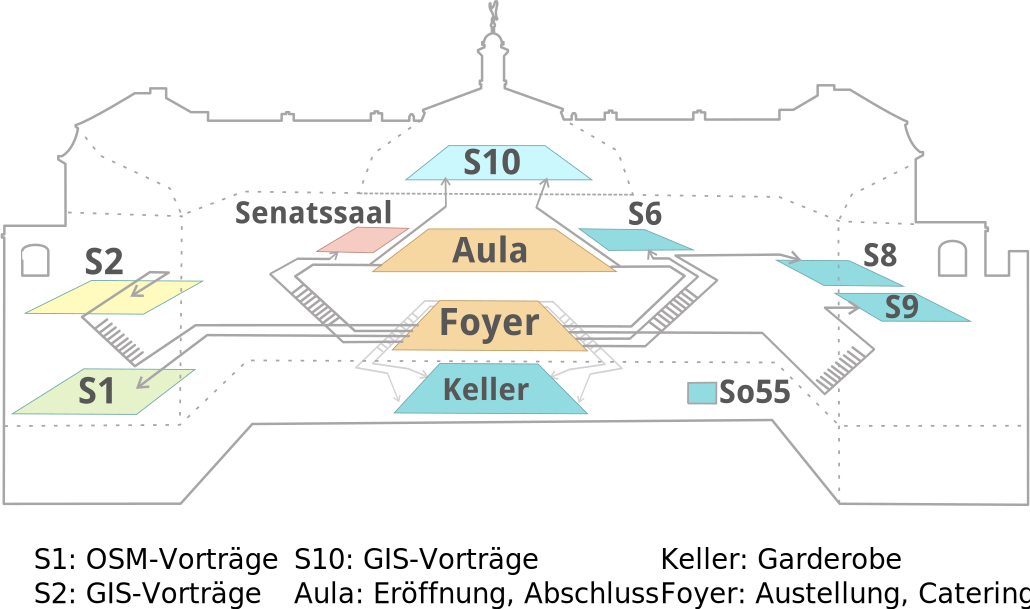
\includegraphics[width=\linewidth]{gebaeudeplan}
	
	{\small Bildquelle: WWU-Grewer, bearbeitet}
\end{landscape}

